
\documentclass[portrait,a0paper,fontscale=0.285]{baposter} % Adjust the font scale/size here

\usepackage[ruled,longend,lined,linesnumbered,portuguese]{algorithm2e}

\usepackage{pgfplots}
\pgfplotsset{compat=1.18} 
\usepackage{capt-of}

\usepackage[utf8]{inputenc}
\usepackage[T1]{fontenc}
\usepackage[brazilian]{babel}
\usepackage{comment}
\usepackage{setspace}

\usepackage{graphicx} % Para usar \resizebox
\usepackage{array}    % Para personalizar colunas de tabelas
\usepackage{colortbl} % Para colorir células da tabela
\usepackage{xcolor}   % Para usar cores

\usepackage{graphicx} % Required for including images
\graphicspath{{figures/}} % Directory in which figures are stored


%\usepackage{algorithm}
%\usepackage[noend]{algpseudocode}
% \usepackage{algorithmic}
%\usepackage[ruled,vlined,boxed]{algorithm2e}
%\usepackage{algpseudocode,algorithm}

\usepackage{scalefnt}
\usepackage{float}
\usepackage[portuguese, ruled, linesnumbered]{algorithm2e}

\usepackage{amsmath} % For typesetting math
\usepackage{amssymb} % Adds new symbols to be used in math mode

\usepackage{booktabs} % Top and bottom rules for tables
\usepackage{enumitem} % Used to reduce itemize/enumerate spacing
\usepackage{palatino} % Use the Palatino font
\usepackage[font=small,labelfont=bf]{caption} % Required for specifying captions to tables and figures
\usepackage{subfig}
\usepackage{tabularx}

\usepackage{multicol} % Required for multiple columns
\setlength{\columnsep}{1.5em} % Slightly increase the space between columns
\setlength{\columnseprule}{0mm} % No horizontal rule between columns

\usepackage{tikz} % Required for flow chart
\usetikzlibrary{shapes,arrows} % Tikz libraries required for the flow chart in the template

\newcommand{\compresslist}{ % Define a command to reduce spacing within itemize/enumerate environments, this is used right after \begin{itemize} or \begin{enumerate}
\setlength{\itemsep}{1pt}
\setlength{\parskip}{0pt}
\setlength{\parsep}{0pt}
}

\definecolor{lightblue}{rgb}{0.145,0.6666,1} % Defines the color used for content box headers

\begin{document}

\begin{poster}
{
headerborder=closed, % Adds a border around the header of content boxes
colspacing=1em, % Column spacing
bgColorOne=white, % Background color for the gradient on the left side of the poster
bgColorTwo=white, % Background color for the gradient on the right side of the poster
borderColor=lightblue, % Border color
headerColorOne=black, % Background color for the header in the content boxes (left side)
headerColorTwo=lightblue, % Background color for the header in the content boxes (right side)
headerFontColor=white, % Text color for the header text in the content boxes
boxColorOne=white, % Background color of the content boxes
textborder=roundedleft, % Format of the border around content boxes, can be: none, bars, coils, triangles, rectangle, rounded, roundedsmall, roundedright or faded
eyecatcher=true, % Set to false for ignoring the left logo in the title and move the title left
headerheight=0.11\textheight, % Height of the header
headershape=roundedright, % Specify the rounded corner in the content box headers, can be: rectangle, small-rounded, roundedright, roundedleft or rounded
headerfont=\Large\bf\textsc, % Large, bold and sans serif font in the headers of content boxes
%textfont={\setlength{\parindent}{1.5em}}, % Uncomment for paragraph indentation
linewidth=2pt % Width of the border lines around content boxes
}
%----------------------------------------------------------------------------------------
%	TITLE SECTION 
%----------------------------------------------------------------------------------------
%
{
\includegraphics[height=10em]{figures/logo-labotim-ufes.png}}
{{\huge Uma meta-heurística para solução do problema da Árvore geradora com número mínimo de vértices d-\textit{branch}}\vspace{0.1em}}
{Marcos Vinícius de Souza Silva e Maria Claudia Silva Boeres \hspace{12pt} \\ Universidade Federal do Espírito Santo}
%{\includegraphics[height=11em]{qrcode.png}}
{
\includegraphics[height=4em]{figures/logo_cnpq.jpg}}
%----------------------------------------------------------------------------------------
%	Resumo
%----------------------------------------------------------------------------------------
\headerbox{\normalsize Resumo}{name=resumo,column=0,row=0,span=3}{
Esta pesquisa aborda métodos da literatura para o problema d-MBV, com ênfase no desenvolvimento do algoritmo construtivo R-PREV, fundamentado em propriedades aleatórias, densidade de grafos e centralidade \textit{PageRank}. Integrado às meta-heurísticas \textit{Multi-Start} e GRASP, o objetivo é aprimorar a qualidade das soluções por meio de múltiplas inicializações aleatórias. As três variações propostas diferem pelo parâmetro $\alpha$ na fase construtiva: \textit{MULTI-START} ($\alpha = 1$), totalmente aleatório; \textit{GRASP-FIXO} ($\alpha = 0.2$), restrito aos $20\%$ melhores candidatos; e \textit{GRASP-REATIVO}, em que $\alpha$ é ajustado dinamicamente conforme o desempenho das iterações. Os experimentos indicaram que todas as abordagens superaram os resultados da literatura, com destaque principal para os resultados obtidos com o método \textit{GRASP-REATIVO}.


%Este trabalho explora métodos da literatura voltados para encontrar soluções eficientes para o problema d-MBV, com foco no estudo e aprimoramento da meta-heurística ILS (Iterated Local Search), do algoritmo construtivo R-BEP (Random Branch Expanding Prim) e da centralidade de grafos \textit{PageRank}. O objetivo central é adaptar e integrar essas abordagens, utilizando a centralidade \textit{PageRank} como uma alternativa inovadora, com a expectativa de melhorar a qualidade das soluções obtidas. As adaptações propostas foram implementadas nas etapas principais do ILS, permitindo avaliar o impacto de diferentes combinações de métodos sobre os resultados e identificar a configuração mais eficaz. O uso do R-BEP contribuiu significativamente para aprimorar a fase construtiva do ILS, enquanto a adoção do \textit{PageRank} no estágio de perturbação se mostrou superior em desempenho em relação à centralidade Grau, com desempenho similar nas demais etapas.
}

%-----------------------------------------------------------------------------------------
% D-MB
%-----------------------------------------------------------------------------------------
\begin{posterbox}[name=modelo,column=0,below=resumo]
{O problema D-MBV}
O objetivo é encontrar uma árvore geradora que minimize a quantidade de vértices com grau superior a $d$, onde $d \geq 2$, em um grafo conexo e não direcionado. Considera-se o grafo original $G = (V_G, E_G)$ e a árvore geradora $T = (V_T, E_T)$, de modo que $V_T = V_G$ e $E_T \subseteq E_G$.


\vspace{-1ex}
\setcaptiontype{figure} % Fake a figure environment
\begin{minipage}{\textwidth}
    \centering
    \subfloat[]{%
        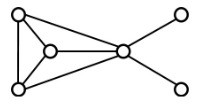
\includegraphics[width=0.27\linewidth]{figures/grafo_g.jpeg}
    }
    \subfloat[]{%
        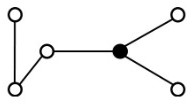
\includegraphics[width=0.27\linewidth]{figures/arvore_t1.jpeg}
    }
    \subfloat[]{%
        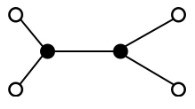
\includegraphics[width=0.27\linewidth]{figures/arvore_t2.jpeg}
    }
    \captionof{figure}{(a) Grafo $G$, (b) e (c) Árvores Geradoras com 1 e 2 vértices \textit{branch}, respectivamente.}
\end{minipage}
\end{posterbox}





\begin{posterbox}[name=conceitos,column=0,below=modelo]
{Estratégias}
\small

Uma síntese das meta-heurísticas implementadas durante esta pesquisa pode ser visualizada na Figura \ref{fig:fluxograma}. O algoritmo construtivo adotado em todas as abordagens foi o R-PREV, desenvolvido neste estudo, enquanto a busca local e a perturbação seguem a adaptação realizada em \cite{silva2024ils}. 

\centering

\captionof{figure}{\scriptsize Fluxograma das combinações de algoritmos aprimoradas e implementadas neste estudo.}
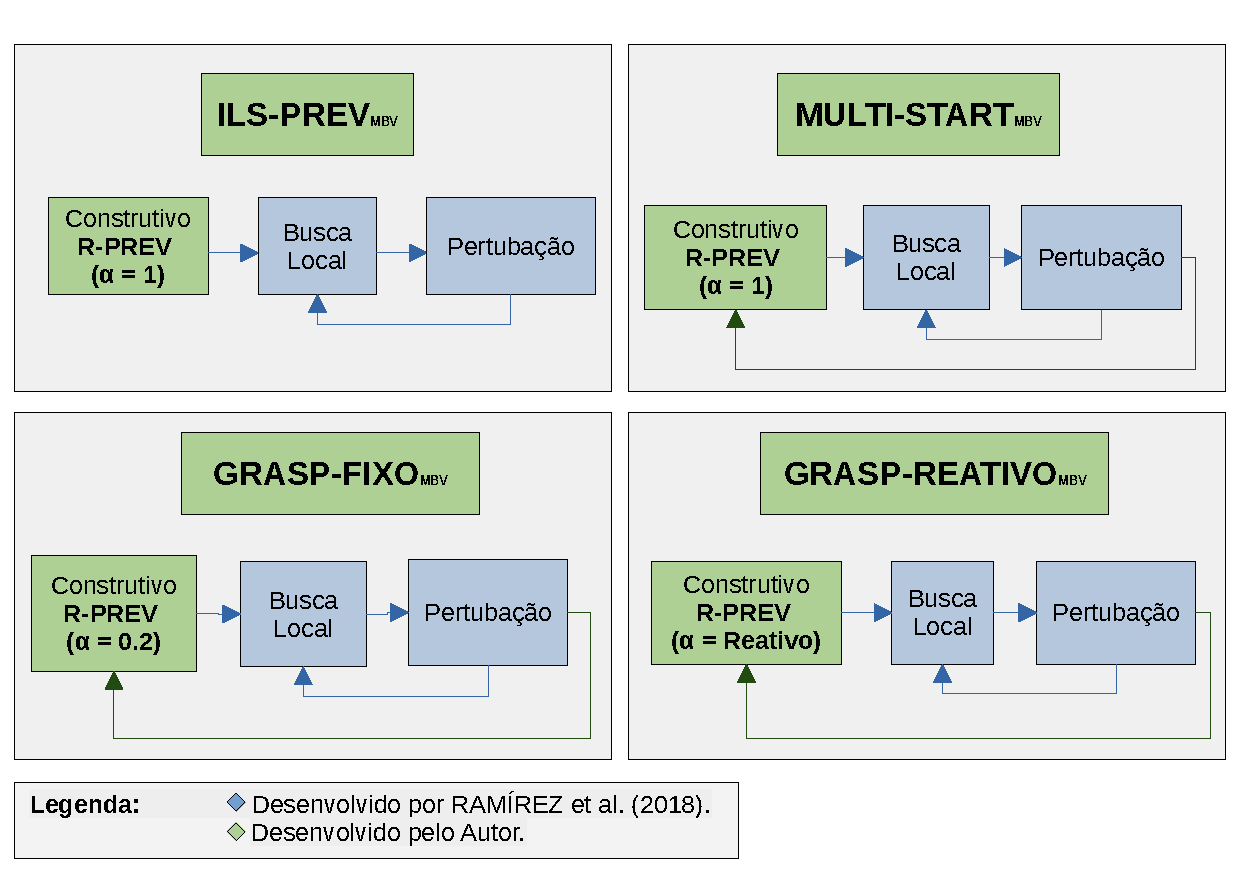
\includegraphics[width=\linewidth]{figures/fluxograma.pdf}

\vspace{-1em}
\caption*{\scriptsize Fonte: Produção do próprio autor.}
\label{fig:fluxograma}
\end{posterbox}






\begin{posterbox}[name=conclusao,column=0,below=conceitos]
{Conclusão}
\small
\begin{itemize}[left=0pt]
    \setlength{\itemsep}{0.1em}
    \setlength{\parindent}{0pt}
    \item O algoritmo construtivo R-PREV foi ligeiramente inferior com apenas uma iteração do laço externo, mas seu valor está em viabilizar as demais meta-heurísticas, por ser rápido e simples de implementar.
    \item As meta-heurísticas tiveram ótimo desempenho: todas as abordagens (MULTI-START, GRASP-FIXO e GRASP-REATIVO) superaram a literatura, com destaque para o GRASP-REATIVO.
    \item É fundamental considerar o trade-off: mais iterações produzem soluções melhores, mas com maior custo computacional.
\end{itemize}
\end{posterbox}


%----------------------------------------------------------------------------------------
% METODOLOGIA
%----------------------------------------------------------------------------------------
\begin{posterbox}[name=metodologia,column=1,below=resumo,span=2]{Metodologia}
\normalsize
Neste estudo, investigou-se como a densidade de um grafo e a centralidade PageRank podem ser exploradas para desenvolver um algoritmo construtivo capaz de prever um conjunto de melhores opções de inicialização. A partir de sorteios realizados nesse conjunto, é gerada uma solução inicial para o problema, conforme descrito no Algoritmo (\ref{alg:rprev}). Esse algoritmo foi incorporado a um \textit{framework} flexível, que permite a integração de diferentes estratégias (MULTI-START e GRASP), facilmente adaptadas por meio de uma variável $\alpha$. Essa variável define o espaço de sorteio da fase construtiva e é ajustada durante a execução. O pseudocódigo do \textit{framework} é apresentado no Algoritmo \ref{alg:frameworkMBV}.
 





%Durante este trabalho, foram analisadas todas as etapas da meta-heurística ILS (Iterated Local Search) proposta por \cite{morenotese:2018} para a resolução do problema $d$-MBV. Os resultados de cada etapa foram estudados separadamente, variações foram propostas, implementadas e avaliadas. Por exemplo, na busca local, foi introduzido um método alternativo para a seleção de soluções vizinhas, e a centralidade foi alterada de grau para \textit{PageRank}. O Algoritmo \ref{alg:ils} apresenta a versão final do ILS modificado, integrando variáveis que determinam quais modificações serão aplicadas em cada rodada de testes, o que possibilita a comparação e o rastreamento da melhor combinação de adaptações realizadas ao longo deste estudo.
\vspace{-0.5cm}


\begin{figure}[H]
\centering
\begin{minipage}{0.5\textwidth}
\scriptsize
\setstretch{0.9} % reduz espaço vertical
\begin{algorithm}[H]
\caption{R-PREV}
\label{alg:rprev}
\SetAlgoLined
\Entrada{Grafo $G = (V, E)$, $\alpha = (0, 1)$.}
\Saida{Árvore Geradora $T = (V, E)$.}
$dbPREV \gets \text{Cálculo-dbPREV}(G)$;
\label{lin:calculo_dbPREV}\\
$(T, B_{\text{T}}, Pontas) \gets \text{Pré-Processamento}(G, dbPREV, \alpha)$;\label{lin:PreProcessamento}\\
\Enqto {$|E_{\text{T}}| < |V_{\text{G}}| - 1$}{ \label{lin:inicioloopRPREV}
    Sorteia um vértice $u \in \text{Pontas}$ com probabilidade proporcional ao seu grau $d(u)$ em $G$;\\
    Sorteia um vizinho $v \in N(u)$ que não forma ciclo em $T$;\\
    Adiciona a aresta $(u, v)$ a $T$;\\
    Atualiza Pontas e $B_{\text{T}}$;
}\label{lin:fimloopRPREV}
\textbf{return} $R$\;
\end{algorithm}
\vspace{-0.5em}
\end{minipage}
\hspace{0.02\textwidth} % reduz espaço horizontal
\begin{minipage}{0.46\textwidth}
\scriptsize
\setstretch{0.5} % reduz espaço vertical
\begin{algorithm}[H]
\caption{Híbrido MBV}
\label{alg:frameworkMBV}
\SetAlgoLined
\Entrada{O grafo $G = (V, E)$, $\alpha = (0, 1)$, $MaxIter$.} \label{lin:EntradaILS}
\Saida{Uma solução válida $T$.}
$T^* \gets \emptyset$\;\label{lin:InicializacaoT*}
\Para{$i = 1$ \textbf{até} $MaxIter$}{ 
    $T_0 \gets RPREV(G, \alpha)$; \label{lin:SolucaoInicialHibrido} \\ 
    $T_{local} \gets Busca\_Local(T_0)$; \label{lin:BuscaLocal1Hibrido}\\
    \Repita{$condicao\ de\ parada\ atendida$}{\label{lin:InicioLoopHibrido}
        $T' \gets Perturbacao(T_{local})$; \label{lin:PertubacaoHibrido}\\
        $T'' \gets Busca\_Local(T')$; \label{lin:BuscaLocal2Hibrido}\\
        $T_{local} \gets Criterio(T_{local}, T'', historia)$; \label{lin:CriterioAceitacaoHibrido}\\   
    }\label{lin:FimLoopHibrido}
    \Se{$T_{local}$ é melhor que $T^*$}{ \label{lin:VerificacaoHibrido}
        $T^* \gets T_{local}$; \label{lin:SalvandoSolucaoHibrido}\\
    }
}
\textbf{return} $T^*$\;
\end{algorithm}
\vspace{-0.5em}
\end{minipage}
\end{figure}




\end{posterbox}

%----------------------------------------------------------------------------------------
% Resultados - DBO
%----------------------------------------------------------------------------------------
\begin{posterbox}[name=resultados,column=1,below=metodologia,span=2]{Resultados}


\begin{figure}[H]
\centering
% --- Superior esquerdo: TEXTO ---
\vspace{-1.2em}
\begin{minipage}[t]{0.48\textwidth}
    \small
Os testes foram realizados em uma máquina com processador Ryzen 5 5600GT, 32 GB de RAM e Linux, abrangendo 525 instâncias. 

A Tabela \ref{tab:resultados_geral} apresenta os resultados gerais, organizados por blocos de iterações do laço externo dos algoritmos. O termo “iterações sem melhorias” indica quantas vezes o algoritmo não conseguiu encontrar uma solução melhor que a atual. A Tabela \ref{tab:resultados_medios_completos} mostra os resultados mínimos para todo o conjunto de instâncias, em que cada linha corresponde à média de cinco grafos. Em ambas as tabelas, os valores destacados em azul representam os melhores resultados. 

A Figura \ref{fig:time_to_target} apresenta um gráfico do tipo \textit{Time to Target}, que avalia o desempenho das heurísticas em função do tempo necessário para atingir uma solução alvo previamente definida.
\vspace{-1.5em}

\end{minipage}
\hfill
% --- Superior direito: TABELA 1 ---
\begin{minipage}[t]{0.48\textwidth}
\centering
\vspace{0.2em}
\captionof{table}{\small Comparação geral entre as meta-heurísticas em diferentes quantidades de iterações.}
\resizebox{1\textwidth}{!}{%
\begin{tabular}{|l|c|c|c|}
\hline
\rowcolor{gray!30}  
\textbf{Informações} & \textbf{MULT-START} & \textbf{GRASP-FIXO} & \textbf{GRASP-REATIVO} \\
\hline

\multicolumn{4}{|c|}{\cellcolor{gray!30}\textbf{20 Iterações sem melhora}} \\
\hline
Tempo total     &9 h 36 min&\cellcolor{blue!20}\textbf{9 h 35 min}&9 h 58 min\\
Exatos          &256&256&\cellcolor{blue!20}\textbf{270}\\
Melhores        &375&369& \cellcolor{blue!20}\textbf{384}\\
\hline

\multicolumn{4}{|c|}{\cellcolor{gray!30}\textbf{50 Iterações sem melhora}} \\
\hline
Tempo total     &\cellcolor{blue!20}\textbf{1 d 7 h 24 min}&1 d 11 h 41 min&1 d 10 h 42 min\\
Exatos          &281&282&\cellcolor{blue!20}\textbf{289}\\
Melhores        &434&446&\cellcolor{blue!20}\textbf{464} \\
\hline

\multicolumn{4}{|c|}{\cellcolor{gray!30}\textbf{100 Iterações sem melhora}} \\
\hline
Tempo total     &2 d 19 h 34 min&2 d 23 h 30 min&\cellcolor{blue!20}\textbf{2 d 16 h 10 min}\\
Exatos          &300&308&\cellcolor{blue!20}\textbf{314}\\
Melhores        &445&454&\cellcolor{blue!20}\textbf{475}\\
\hline

\end{tabular}}
\caption*{\scriptsize Fonte: Produção do próprio autor.}
\label{tab:resultados_geral}
\end{minipage}

\vspace{1em}

% --- Inferior esquerdo: GRÁFICOS ---
\begin{minipage}[t]{0.48\textwidth}
\centering
\begin{figure}[ht]
\centering
\caption{\small Comparação entre diferentes instâncias sobre o comportamento das meta-heurísticas implementadas.}
\vspace{-0.5em}

\begin{minipage}{0.48\textwidth}
    \centering
    % --- Primeiro gráfico ---
    \begin{tikzpicture}
    \begin{axis}
    [
    width=1.3\textwidth,
    height=1\textwidth,
    xlabel={\tiny Tempo (s)},
    ylabel={\tiny Fração de execuções},
    title={\tiny Instância: 40 vértices, 81 arestas, alvo = 0},
    ticklabel style={/pgfplots/ylabel shift=0.5ex}, % move todos os números
    yticklabel style={xshift=-0.4ex}, % afasta os números do eixo y
    xticklabel style={yshift=-0.4ex},  % afasta os números do eixo x
    xlabel style={yshift=-0.4ex},
    ymin=0,
    xmin=0,
    xtick={0.0,0.2,0.4,0.6,0.8,1.0},
    xticklabels={
            \tiny 0.0,
            \tiny 0.2,
            \tiny 0.4,
            \tiny 0.6,
            \tiny 0.8,
            \tiny 1.0},
    ytick={0.0,0.2,0.4,0.6,0.8,1.0},
    yticklabels={
            \tiny 0.0,
            \tiny 0.2,
            \tiny 0.4,
            \tiny 0.6,
            \tiny 0.8,
            \tiny 1.0},
    legend pos=south east,
    grid=major,
    legend to name=legendaMetodos, % salva a legenda
    legend columns=3,
    legend style={
        font=\scriptsize,   % <-- muda o tamanho da fonte
        at={(0.5,-0.2)},    % posiciona abaixo do gráfico
        anchor=north,
        legend columns=3    % número de colunas
    }
    ]

% Linha vermelha - Mult Start (N=100 execuções)
\addplot+[
    mark=none,
    thick,
    red,
] coordinates {
    (0,0) (0.000632,0.01) (0.00181,0.02) (0.002331,0.03) (0.004736,0.04) (0.005643,0.05) (0.006406,0.06) (0.006724,0.07) (0.007706,0.08) (0.010621,0.09) (0.013021,0.1) (0.017736,0.11) (0.020646,0.12) (0.023954,0.13) (0.024236,0.14) (0.027313,0.15) (0.029496,0.16) (0.031547,0.17) (0.037815,0.18) (0.038277,0.19) (0.038553,0.2) (0.039101,0.21) (0.039656,0.22) (0.043027,0.23) (0.044767,0.24) (0.045467,0.25) (0.049114,0.26) (0.053158,0.27) (0.056794,0.28) (0.057544,0.29) (0.058977,0.3) (0.061211,0.31) (0.065408,0.32) (0.067346,0.33) (0.0801,0.34) (0.081401,0.35) (0.088155,0.36) (0.090264,0.37) (0.09028,0.38) (0.091681,0.39) (0.094101,0.4) (0.098676,0.41) (0.099907,0.42) (0.099922,0.43) (0.100684,0.44) (0.101936,0.45) (0.103795,0.46) (0.1102,0.47) (0.117659,0.48) (0.120744,0.49) (0.121632,0.5) (0.128157,0.51) (0.130645,0.52) (0.131343,0.53) (0.135287,0.54) (0.153573,0.55) (0.160806,0.56) (0.161366,0.57) (0.173776,0.58) (0.175115,0.59) (0.175372,0.6) (0.198607,0.61) (0.216443,0.62) (0.219741,0.63) (0.225004,0.64) (0.232487,0.65) (0.232657,0.66) (0.243291,0.67) (0.24891,0.68) (0.258715,0.69) (0.26353,0.7) (0.278519,0.71) (0.281222,0.72) (0.282823,0.73) (0.303047,0.74) (0.303923,0.75) (0.305949,0.76) (0.310113,0.77) (0.315213,0.78) (0.35106,0.79) (0.356332,0.8) (0.37048,0.81) (0.37592,0.82) (0.385782,0.83) (0.388632,0.84) (0.392375,0.85) (0.413208,0.86) (0.436497,0.87) (0.490144,0.88) (0.494925,0.89) (0.519258,0.9) (0.523873,0.91) (0.533659,0.92) (0.557047,0.93) (0.575165,0.94) (0.586183,0.95) (0.625416,0.96) (0.6419,0.97) (0.676312,0.98) (0.715766,0.99) (1.02488,1.0)
};
\addlegendentry{\tiny MULTI-START}

% Linha azul - GRASP_FIXO (N=100 execuções)
\addplot+[
    mark=none,
    thick,
    blue,
] coordinates {
    (0,0) (0.001834,0.01) (0.003413,0.02) (0.003629,0.03) (0.00415,0.04) (0.004412,0.05) (0.007022,0.06) (0.007975,0.07) (0.0087,0.08) (0.011698,0.09) (0.01203,0.1) (0.012376,0.11) (0.012958,0.12) (0.01316,0.13) (0.013761,0.14) (0.014708,0.15) (0.015065,0.16) (0.017188,0.17) (0.020347,0.18) (0.022473,0.19) (0.022772,0.2) (0.024155,0.21) (0.026271,0.22) (0.026405,0.23) (0.029907,0.24) (0.031963,0.25) (0.033053,0.26) (0.03692,0.27) (0.040755,0.28) (0.040976,0.29) (0.041333,0.3) (0.041859,0.31) (0.041944,0.32) (0.043949,0.33) (0.047048,0.34) (0.048295,0.35) (0.049148,0.36) (0.05053,0.37) (0.058357,0.38) (0.059303,0.39) (0.059468,0.4) (0.061536,0.41) (0.064294,0.42) (0.06445,0.43) (0.065682,0.44) (0.066048,0.45) (0.070253,0.46) (0.070667,0.47) (0.072294,0.48) (0.075498,0.49) (0.07635,0.5) (0.081435,0.51) (0.081785,0.52) (0.087967,0.53) (0.089238,0.54) (0.090885,0.55) (0.092048,0.56) (0.095351,0.57) (0.096038,0.58) (0.101064,0.59) (0.103583,0.6) (0.117967,0.61) (0.119292,0.62) (0.120611,0.63) (0.121279,0.64) (0.126164,0.65) (0.127061,0.66) (0.127889,0.67) (0.12834,0.68) (0.131015,0.69) (0.142832,0.7) (0.143148,0.71) (0.145576,0.72) (0.157374,0.73) (0.161647,0.74) (0.174943,0.75) (0.179176,0.76) (0.182134,0.77) (0.18569,0.78) (0.196958,0.79) (0.202207,0.8) (0.203656,0.81) (0.204899,0.82) (0.207748,0.83) (0.211467,0.84) (0.212869,0.85) (0.215562,0.86) (0.224717,0.87) (0.234477,0.88) (0.239409,0.89) (0.265007,0.9) (0.26622,0.91) (0.281357,0.92) (0.327259,0.93) (0.329013,0.94) (0.339574,0.95) (0.347873,0.96) (0.351706,0.97) (0.355585,0.98) (0.435194,0.99) (0.482585,1.0)
};
\addlegendentry{\tiny GRASP-FIXO}

% Linha verde - GRASP_REATIVO (N=100 execuções)
\addplot+[
    mark=none,
    thick,
    green!60!black,
] coordinates {
    (0,0) (0.002713,0.01) (0.00286,0.02) (0.004043,0.03) (0.006405,0.04) (0.007703,0.05) (0.007761,0.06) (0.008052,0.07) (0.009182,0.08) (0.012158,0.09) (0.012949,0.1) (0.012971,0.11) (0.013276,0.12) (0.015629,0.13) (0.015858,0.14) (0.018092,0.15) (0.018886,0.16) (0.020239,0.17) (0.021942,0.18) (0.026126,0.19) (0.027664,0.2) (0.028625,0.21) (0.028834,0.22) (0.031181,0.23) (0.034108,0.24) (0.038723,0.25) (0.039354,0.26) (0.040339,0.27) (0.04066,0.28) (0.043965,0.29) (0.045218,0.3) (0.047969,0.31) (0.048268,0.32) (0.048305,0.33) (0.053441,0.34) (0.054925,0.35) (0.0551,0.36) (0.055721,0.37) (0.058997,0.38) (0.060107,0.39) (0.061206,0.4) (0.063514,0.41) (0.066584,0.42) (0.067585,0.43) (0.068903,0.44) (0.069387,0.45) (0.070213,0.46) (0.071002,0.47) (0.072006,0.48) (0.072488,0.49) (0.072979,0.5) (0.073244,0.51) (0.073601,0.52) (0.074246,0.53) (0.076044,0.54) (0.079686,0.55) (0.080191,0.56) (0.08031,0.57) (0.082714,0.58) (0.082867,0.59) (0.087573,0.6) (0.088473,0.61) (0.091859,0.62) (0.094287,0.63) (0.095868,0.64) (0.09657,0.65) (0.099191,0.66) (0.102741,0.67) (0.103927,0.68) (0.103936,0.69) (0.105378,0.7) (0.105471,0.71) (0.107861,0.72) (0.112348,0.73) (0.11383,0.74) (0.118859,0.75) (0.124825,0.76) (0.135069,0.77) (0.15112,0.78) (0.15156,0.79) (0.153516,0.8) (0.155957,0.81) (0.15994,0.82) (0.168003,0.83) (0.173467,0.84) (0.176268,0.85) (0.180609,0.86) (0.187561,0.87) (0.214536,0.88) (0.215297,0.89) (0.236042,0.9) (0.254049,0.91) (0.261351,0.92) (0.277943,0.93) (0.279339,0.94) (0.289929,0.95) (0.291039,0.96) (0.303858,0.97) (0.55991,1.0)
};\addlegendentry{\tiny GRASP-REATIVO}
    \end{axis}
    \end{tikzpicture}
\end{minipage}
\hfill
\begin{minipage}{0.48\textwidth}
    \centering
    % --- Terceiro gráfico ---
    \begin{tikzpicture}
    \begin{axis}
    [
    width=1.3\textwidth,
    height=1\textwidth,
    xlabel={\tiny Tempo (s)},
    ylabel={\tiny Fração de execuções},
    title={\tiny Instância: 100 vértices, 174 arestas, alvo = 8},
    ticklabel style={/pgfplots/ylabel shift=0.5ex}, % move todos os números
    yticklabel style={xshift=-0.4ex}, % afasta os números do eixo y
    xticklabel style={yshift=-0.4ex},  % afasta os números do eixo x
    xlabel style={yshift=-0.4ex},
    ymin=0, ymax=1.05,
    xmin=0, xmax = 100,
    xtick={0,20,40,60,80,100},
    xticklabels={
            \tiny 0,
            \tiny 20,
            \tiny 40,
            \tiny 60,
            \tiny 80,
            \tiny 100},
    ytick={0.0,0.2,0.4,0.6,0.8,1.0},
    yticklabels={
            \tiny 0.0,
            \tiny 0.2,
            \tiny 0.4,
            \tiny 0.6,
            \tiny 0.8,
            \tiny 1.0},
    legend pos=south east,
    grid=major,
    ]

% Linha vermelha - Mult Start (N=100 execuções)
\addplot+[
    mark=none,
    thick,
    red,
] coordinates {
    (0,0) (0.068223,0.01) (0.591313,0.02) (0.638326,0.03) (0.767011,0.04) (0.959076,0.05) (1.00404,0.06) (1.01041,0.07) (1.24452,0.08) (1.51633,0.09) (1.63983,0.1) (1.79963,0.11) (1.96049,0.12) (2.08652,0.13) (2.32771,0.14) (2.48226,0.15) (2.55205,0.16) (2.7564,0.17) (2.89128,0.18) (2.89862,0.19) (2.98068,0.2) (3.17621,0.21) (3.31436,0.22) (3.43421,0.23) (3.64078,0.24) (3.72922,0.25) (3.79823,0.26) (4.13906,0.27) (4.31255,0.28) (4.64335,0.29) (4.71654,0.3) (5.14706,0.31) (5.14726,0.32) (5.64291,0.33) (5.68802,0.34) (5.77941,0.35) (5.92676,0.36) (6.10329,0.37) (6.11102,0.38) (6.14603,0.39) (6.65341,0.4) (6.9343,0.41) (7.1368,0.42) (7.24032,0.43) (7.43327,0.44) (7.62952,0.45) (7.79035,0.46) (8.54075,0.47) (8.73445,0.48) (8.83442,0.49) (8.83558,0.5) (8.9028,0.51) (9.64681,0.52) (9.68175,0.53) (9.81778,0.54) (10.6163,0.55) (10.9654,0.56) (11.0524,0.57) (11.0541,0.58) (11.3633,0.59) (11.4596,0.6) (13.5798,0.61) (13.9199,0.62) (14.1514,0.63) (15.4169,0.64) (15.8871,0.65) (16.7213,0.66) (17.9511,0.67) (19.3207,0.68) (20.0869,0.69) (20.1168,0.7) (20.9151,0.71) (21.4003,0.72) (21.8477,0.73) (22.0087,0.74) (22.2713,0.75) (22.6299,0.76) (23.0686,0.77) (23.0843,0.78) (25.0249,0.79) (25.6839,0.8) (27.6935,0.81) (28.0048,0.82) (30.4495,0.83) (31.2064,0.84) (32.0097,0.85) (33.1858,0.86) (33.8709,0.87) (34.8258,0.88) (36.4367,0.89) (36.4523,0.9) (36.9591,0.91) (44.0267,0.92) (44.9602,0.93) (59.5709,0.94) (60.1774,0.95) (67.5787,0.96) (69.9369,0.97) (72.4247,0.98) (90.4803,0.99) (91.0376,1.0)
};

% Linha azul - GRASP_FIXO (N=100 execuções)
\addplot+[
    mark=none,
    thick,
    blue,
] coordinates {
    (0,0) (0.070778,0.01) (0.442093,0.02) (0.635793,0.03) (0.801707,0.04) (0.917302,0.05) (0.977615,0.06) (1.01541,0.07) (1.02089,0.08) (1.0449,0.09) (1.22588,0.1) (1.26657,0.11) (1.62545,0.12) (1.74241,0.13) (1.89432,0.14) (1.90482,0.15) (2.25505,0.16) (2.40892,0.17) (2.54917,0.18) (2.58329,0.19) (2.99755,0.2) (3.31618,0.21) (3.42051,0.22) (3.72941,0.23) (3.75277,0.24) (3.8583,0.25) (4.15855,0.26) (4.64359,0.27) (4.72085,0.28) (4.90284,0.29) (5.02319,0.3) (5.03122,0.31) (5.23319,0.32) (5.81078,0.33) (5.89867,0.34) (6.05664,0.35) (6.13768,0.36) (6.30059,0.37) (6.55993,0.38) (6.8601,0.39) (7.09175,0.4) (7.34885,0.41) (7.3505,0.42) (7.57947,0.43) (7.66769,0.44) (7.70167,0.45) (7.79026,0.46) (8.14849,0.47) (8.54669,0.48) (9.08149,0.49) (9.09763,0.5) (9.11144,0.51) (9.38931,0.52) (9.98608,0.53) (10.0506,0.54) (10.1066,0.55) (10.3071,0.56) (10.8372,0.57) (10.9733,0.58) (11.1146,0.59) (11.2317,0.6) (11.5742,0.61) (12.0013,0.62) (14.2798,0.63) (14.3566,0.64) (14.5726,0.65) (15.8501,0.66) (16.3818,0.67) (17.4058,0.68) (17.8797,0.69) (18.1473,0.7) (18.3682,0.71) (20.3137,0.72) (20.8484,0.73) (21.1904,0.74) (21.9987,0.75) (22.1973,0.76) (22.5045,0.77) (22.8594,0.78) (22.979,0.79) (23.5833,0.8) (23.6203,0.81) (26.0233,0.82) (26.289,0.83) (28.4619,0.84) (28.5186,0.85) (33.0747,0.86) (33.1046,0.87) (34.2005,0.88) (34.549,0.89) (34.7187,0.9) (36.7412,0.91) (36.8882,0.92) (39.6589,0.93) (45.2977,0.94) (46.1436,0.95) (61.4674,0.96) (67.5706,0.97) (70.693,0.98) (92.8788,0.99) (93.1456,1.0)
};

% Linha verde - GRASP_REATIVO (N=100 execuções)
\addplot+[
    mark=none,
    thick,
    green!60!black,
] coordinates {
    (0,0) (0.1844,0.01) (0.230932,0.02) (0.365424,0.03) (0.391309,0.04) (0.481846,0.05) (0.496277,0.06) (0.499065,0.07) (0.642898,0.08) (0.665872,0.09) (0.677321,0.1) (0.736916,0.11) (0.748171,0.12) (1.03131,0.13) (1.04113,0.14) (1.32964,0.15) (1.51109,0.16) (1.56523,0.17) (1.5756,0.18) (1.58742,0.19) (1.7307,0.2) (1.75043,0.21) (1.83169,0.22) (2.02502,0.23) (2.07662,0.24) (2.08152,0.25) (2.16004,0.26) (2.21083,0.27) (2.40639,0.28) (2.53731,0.29) (2.63059,0.3) (2.63575,0.31) (2.70445,0.32) (2.73231,0.33) (2.89515,0.34) (3.29716,0.35) (3.69656,0.36) (3.85306,0.37) (3.93738,0.38) (3.94288,0.39) (4.0963,0.4) (4.35503,0.41) (4.591,0.42) (4.61621,0.43) (4.63739,0.44) (4.6757,0.45) (4.89462,0.46) (5.024,0.47) (5.10556,0.48) (5.26791,0.49) (5.30959,0.5) (5.36969,0.51) (5.45175,0.52) (5.56989,0.53) (5.98844,0.54) (6.04625,0.55) (6.22696,0.56) (6.39407,0.57) (6.59535,0.58) (6.63777,0.59) (6.66101,0.6) (6.69842,0.61) (6.75961,0.62) (7.22689,0.63) (7.33906,0.64) (7.5307,0.65) (7.61527,0.66) (7.71622,0.67) (8.22522,0.68) (8.60228,0.69) (8.70456,0.7) (8.95307,0.71) (8.96821,0.72) (9.15192,0.73) (9.27409,0.74) (9.51925,0.75) (9.78642,0.76) (9.78866,0.77) (10.2229,0.78) (10.6394,0.79) (10.6414,0.8) (10.93,0.81) (10.9818,0.82) (11.409,0.83) (11.6451,0.84) (12.1757,0.85) (13.4506,0.86) (13.8229,0.87) (14.3699,0.88) (15.3619,0.89) (15.3924,0.9) (16.8528,0.91) (19.4951,0.92) (19.9244,0.93) (22.2007,0.94) (24.5481,0.95) (25.101,0.96) (26.6065,0.97) (28.8192,0.98) (28.9581,0.99) (29.321,1.0)
};
    \end{axis}
    \end{tikzpicture}
\end{minipage}
\ref{legendaMetodos}
\caption*{\tiny Fonte: Produção do próprio autor.}
\label{fig:time_to_target}
\end{figure}



\end{minipage}
\hfill
% --- Inferior direito: TABELA 2 ---
\begin{minipage}[t]{0.48\textwidth}

\centering
%\caption{\scriptsize Média dos resultados mínimos.}
\captionof{table}{\small Média dos resultados mínimos.}
\vspace{-0.8em}
\resizebox{\textwidth}{!}{%
\begin{tabular}{|cc|c|c|c|c|c|c|}
\hline
\rowcolor{gray!30} \textbf{$n'$} & \textbf{$m'$} & \textbf{Exato} & \textbf{ILS} & \textbf{ILS+} & \textbf{MULTI-START} & \textbf{GRASP-FIXO} & \textbf{GRASP-REATIVO} \\
\hline
20  & 41.8  & 0.76  & 0.80  & 0.80  & \cellcolor{blue!20}0.76  & \cellcolor{blue!20}0.76  & \cellcolor{blue!20}0.76  \\
40  & 70.8  & 2.76  & 3.00  & 2.96  & 2.84  & \cellcolor{blue!20}2.80  & 2.88  \\
60  & 95.0  & 6.30  & 6.70  & 6.72  & \cellcolor{blue!20}6.44  & 6.56  & 6.48  \\
80  & 119.8 & 9.24  & 9.60  & 9.84  & \cellcolor{blue!20}9.28  & 9.32  & \cellcolor{blue!20}9.28  \\
100 & 144.0 & 13.32 & 13.80 & 14.16 & \cellcolor{blue!20}13.40 & \cellcolor{blue!20}13.40 & 13.44 \\
120 & 168.8 & 17.50 & 18.20 & 18.12 & 17.64 & \cellcolor{blue!20}17.60 & \cellcolor{blue!20}17.60 \\
140 & 193.0 & 20.92 & 21.60 & 21.80 & \cellcolor{blue!20}21.08 & 21.12 & \cellcolor{blue!20}21.08 \\
160 & 217.8 & 25.00 & 25.90 & 26.04 & \cellcolor{blue!20}25.32 & 25.48 & \cellcolor{blue!20}25.32 \\
180 & 242.0 & 29.08 & 30.20 & 30.12 & 29.40 & \cellcolor{blue!20}29.36 & 29.48 \\
200 & 266.8 & 32.64 & 33.80 & 33.64 & 33.08 & 33.08 & \cellcolor{blue!20}33.00 \\
250 & 321.0 & 44.60 & 45.70 & 45.96 & 45.12 & 45.12 & \cellcolor{blue!20}45.08 \\
300 & 380.0 & 57.36 & 58.70 & 58.76 & 58.00 & \cellcolor{blue!20}57.88 & 58.00 \\
350 & 434.8 & 68.56 & 70.10 & 70.20 & 69.28 & \cellcolor{blue!20}69.12 & 69.24 \\
400 & 489.0 & 81.84 & 83.50 & 83.92 & 82.64 & \cellcolor{blue!20}82.56 & \cellcolor{blue!20}82.56 \\
450 & 548.0 & 93.36 & 95.30 & 95.36 & 94.28 & 94.20 & \cellcolor{blue!20}94.16 \\
500 & 602.8 & 106.72& 108.60& 109.08& 107.84& 107.80& \cellcolor{blue!20}107.60\\
600 & 711.8 & 153.24& 155.16& 155.40& 154.52& \cellcolor{blue!20}154.44& 154.56\\
700 & 820.8 & 182.12& 184.40& 184.28& 183.40& 183.56& \cellcolor{blue!20}183.32\\
800 & 930.0 & 210.40& 212.92& 212.88& 212.20& 212.16& \cellcolor{blue!20}212.00\\
900 & 1034.0 & 241.72& 244.24& 244.60& 243.80& \cellcolor{blue!20}243.72& \cellcolor{blue!20}243.72\\
1000 & 1143.0 & 271.92& 274.76& 274.76& \cellcolor{blue!20}273.92& \cellcolor{blue!20}273.92& \cellcolor{blue!20}243.72\\
\hline
\end{tabular}}
\caption*{\scriptsize Fonte: Produção do próprio autor.}
\label{tab:resultados_medios_completos}
\end{minipage}

\end{figure}





\begin{comment}
\begin{center}
    \begin{minipage}{0.48\linewidth}
    \small
    \noindent % Remove o recuo da primeira linha
    Os testes foram realizados em uma máquina com processador Ryzen 5 5600GT, 32 GB de RAM e Linux, abrangendo 525 instâncias. A Tabela \ref{tab:ils-complete} apresenta a média dos resultados por grupo de instâncias com o mesmo número de vértices, enquanto a Tabela \ref{tab:ils-geral} mostra os resultados gerais, os melhores resultados estão destacados em azul.

    \begin{figure}[ht]
        \centering
        \caption{\small Comparação entre diferentes instâncias sobre o comportamento das meta-heurísticas implementadas.}
        
        \begin{minipage}{0.48\textwidth}
            \centering
            % --- Primeiro gráfico ---
            \begin{tikzpicture}
            \begin{axis}
            [
            width=0.95\textwidth,
            height=0.65\textwidth,
            xlabel={\footnotesize Tempo (s)},
            ylabel={\footnotesize Fração de execuções},
            title={\footnotesize Instância: 40 vértices, 81 arestas, alvo = 0},
            ymin=0,
            xmin=0,
            xtick={0.0,0.2,0.4,0.6,0.8,1.0},
            xticklabels={
                    \footnotesize 0.0,
                    \footnotesize 0.2,
                    \footnotesize 0.4,
                    \footnotesize 0.6,
                    \footnotesize 0.8,
                    \footnotesize 1.0},
            ytick={0.0,0.2,0.4,0.6,0.8,1.0},
            yticklabels={
                    \footnotesize 0.0,
                    \footnotesize 0.2,
                    \footnotesize 0.4,
                    \footnotesize 0.6,
                    \footnotesize 0.8,
                    \footnotesize 1.0},
            legend pos=south east,
            grid=major,
            legend to name=legendaMetodos, % salva a legenda
            legend columns=3,
            legend style={/tikz/every even column/.append style={column sep=1cm}}
        ]
        
        % Linha vermelha - Mult Start (N=100 execuções)
        \addplot+[
            mark=none,
            thick,
            red,
        ] coordinates {
            (0,0) (0.000632,0.01) (0.00181,0.02) (0.002331,0.03) (0.004736,0.04) (0.005643,0.05) (0.006406,0.06) (0.006724,0.07) (0.007706,0.08) (0.010621,0.09) (0.013021,0.1) (0.017736,0.11) (0.020646,0.12) (0.023954,0.13) (0.024236,0.14) (0.027313,0.15) (0.029496,0.16) (0.031547,0.17) (0.037815,0.18) (0.038277,0.19) (0.038553,0.2) (0.039101,0.21) (0.039656,0.22) (0.043027,0.23) (0.044767,0.24) (0.045467,0.25) (0.049114,0.26) (0.053158,0.27) (0.056794,0.28) (0.057544,0.29) (0.058977,0.3) (0.061211,0.31) (0.065408,0.32) (0.067346,0.33) (0.0801,0.34) (0.081401,0.35) (0.088155,0.36) (0.090264,0.37) (0.09028,0.38) (0.091681,0.39) (0.094101,0.4) (0.098676,0.41) (0.099907,0.42) (0.099922,0.43) (0.100684,0.44) (0.101936,0.45) (0.103795,0.46) (0.1102,0.47) (0.117659,0.48) (0.120744,0.49) (0.121632,0.5) (0.128157,0.51) (0.130645,0.52) (0.131343,0.53) (0.135287,0.54) (0.153573,0.55) (0.160806,0.56) (0.161366,0.57) (0.173776,0.58) (0.175115,0.59) (0.175372,0.6) (0.198607,0.61) (0.216443,0.62) (0.219741,0.63) (0.225004,0.64) (0.232487,0.65) (0.232657,0.66) (0.243291,0.67) (0.24891,0.68) (0.258715,0.69) (0.26353,0.7) (0.278519,0.71) (0.281222,0.72) (0.282823,0.73) (0.303047,0.74) (0.303923,0.75) (0.305949,0.76) (0.310113,0.77) (0.315213,0.78) (0.35106,0.79) (0.356332,0.8) (0.37048,0.81) (0.37592,0.82) (0.385782,0.83) (0.388632,0.84) (0.392375,0.85) (0.413208,0.86) (0.436497,0.87) (0.490144,0.88) (0.494925,0.89) (0.519258,0.9) (0.523873,0.91) (0.533659,0.92) (0.557047,0.93) (0.575165,0.94) (0.586183,0.95) (0.625416,0.96) (0.6419,0.97) (0.676312,0.98) (0.715766,0.99) (1.02488,1.0)
        };
        \addlegendentry{\footnotesize MULTI-START}
        
        % Linha azul - GRASP_FIXO (N=100 execuções)
        \addplot+[
            mark=none,
            thick,
            blue,
        ] coordinates {
            (0,0) (0.001834,0.01) (0.003413,0.02) (0.003629,0.03) (0.00415,0.04) (0.004412,0.05) (0.007022,0.06) (0.007975,0.07) (0.0087,0.08) (0.011698,0.09) (0.01203,0.1) (0.012376,0.11) (0.012958,0.12) (0.01316,0.13) (0.013761,0.14) (0.014708,0.15) (0.015065,0.16) (0.017188,0.17) (0.020347,0.18) (0.022473,0.19) (0.022772,0.2) (0.024155,0.21) (0.026271,0.22) (0.026405,0.23) (0.029907,0.24) (0.031963,0.25) (0.033053,0.26) (0.03692,0.27) (0.040755,0.28) (0.040976,0.29) (0.041333,0.3) (0.041859,0.31) (0.041944,0.32) (0.043949,0.33) (0.047048,0.34) (0.048295,0.35) (0.049148,0.36) (0.05053,0.37) (0.058357,0.38) (0.059303,0.39) (0.059468,0.4) (0.061536,0.41) (0.064294,0.42) (0.06445,0.43) (0.065682,0.44) (0.066048,0.45) (0.070253,0.46) (0.070667,0.47) (0.072294,0.48) (0.075498,0.49) (0.07635,0.5) (0.081435,0.51) (0.081785,0.52) (0.087967,0.53) (0.089238,0.54) (0.090885,0.55) (0.092048,0.56) (0.095351,0.57) (0.096038,0.58) (0.101064,0.59) (0.103583,0.6) (0.117967,0.61) (0.119292,0.62) (0.120611,0.63) (0.121279,0.64) (0.126164,0.65) (0.127061,0.66) (0.127889,0.67) (0.12834,0.68) (0.131015,0.69) (0.142832,0.7) (0.143148,0.71) (0.145576,0.72) (0.157374,0.73) (0.161647,0.74) (0.174943,0.75) (0.179176,0.76) (0.182134,0.77) (0.18569,0.78) (0.196958,0.79) (0.202207,0.8) (0.203656,0.81) (0.204899,0.82) (0.207748,0.83) (0.211467,0.84) (0.212869,0.85) (0.215562,0.86) (0.224717,0.87) (0.234477,0.88) (0.239409,0.89) (0.265007,0.9) (0.26622,0.91) (0.281357,0.92) (0.327259,0.93) (0.329013,0.94) (0.339574,0.95) (0.347873,0.96) (0.351706,0.97) (0.355585,0.98) (0.435194,0.99) (0.482585,1.0)
        };
        \addlegendentry{\footnotesize GRASP-FIXO}
        
        % Linha verde - GRASP_REATIVO (N=100 execuções)
        \addplot+[
            mark=none,
            thick,
            green!60!black,
        ] coordinates {
            (0,0) (0.002713,0.01) (0.00286,0.02) (0.004043,0.03) (0.006405,0.04) (0.007703,0.05) (0.007761,0.06) (0.008052,0.07) (0.009182,0.08) (0.012158,0.09) (0.012949,0.1) (0.012971,0.11) (0.013276,0.12) (0.015629,0.13) (0.015858,0.14) (0.018092,0.15) (0.018886,0.16) (0.020239,0.17) (0.021942,0.18) (0.026126,0.19) (0.027664,0.2) (0.028625,0.21) (0.028834,0.22) (0.031181,0.23) (0.034108,0.24) (0.038723,0.25) (0.039354,0.26) (0.040339,0.27) (0.04066,0.28) (0.043965,0.29) (0.045218,0.3) (0.047969,0.31) (0.048268,0.32) (0.048305,0.33) (0.053441,0.34) (0.054925,0.35) (0.0551,0.36) (0.055721,0.37) (0.058997,0.38) (0.060107,0.39) (0.061206,0.4) (0.063514,0.41) (0.066584,0.42) (0.067585,0.43) (0.068903,0.44) (0.069387,0.45) (0.070213,0.46) (0.071002,0.47) (0.072006,0.48) (0.072488,0.49) (0.072979,0.5) (0.073244,0.51) (0.073601,0.52) (0.074246,0.53) (0.076044,0.54) (0.079686,0.55) (0.080191,0.56) (0.08031,0.57) (0.082714,0.58) (0.082867,0.59) (0.087573,0.6) (0.088473,0.61) (0.091859,0.62) (0.094287,0.63) (0.095868,0.64) (0.09657,0.65) (0.099191,0.66) (0.102741,0.67) (0.103927,0.68) (0.103936,0.69) (0.105378,0.7) (0.105471,0.71) (0.107861,0.72) (0.112348,0.73) (0.11383,0.74) (0.118859,0.75) (0.124825,0.76) (0.135069,0.77) (0.15112,0.78) (0.15156,0.79) (0.153516,0.8) (0.155957,0.81) (0.15994,0.82) (0.168003,0.83) (0.173467,0.84) (0.176268,0.85) (0.180609,0.86) (0.187561,0.87) (0.214536,0.88) (0.215297,0.89) (0.236042,0.9) (0.254049,0.91) (0.261351,0.92) (0.277943,0.93) (0.279339,0.94) (0.289929,0.95) (0.291039,0.96) (0.303858,0.97) (0.55991,1.0)
        };\addlegendentry{\footnotesize GRASP-REATIVO}
            \end{axis}
            \end{tikzpicture}
        \end{minipage}
        \hfill
                
        \begin{minipage}{0.48\textwidth}
            \centering
            % --- Terceiro gráfico ---
            \begin{tikzpicture}
            \begin{axis}
            [
            width=0.95\textwidth,
            height=0.65\textwidth,
            xlabel={\footnotesize Tempo (s)},
            ylabel={\footnotesize Fração de execuções},
            title={\footnotesize Instância: 100 vértices, 174 arestas, alvo = 8},
            ymin=0, ymax=1.05,
            xmin=0, xmax = 100,
            xtick={0,20,40,60,80,100},
            xticklabels={
                    \footnotesize 0,
                    \footnotesize 20,
                    \footnotesize 40,
                    \footnotesize 60,
                    \footnotesize 80,
                    \footnotesize 100},
            ytick={0.0,0.2,0.4,0.6,0.8,1.0},
            yticklabels={
                    \footnotesize 0.0,
                    \footnotesize 0.2,
                    \footnotesize 0.4,
                    \footnotesize 0.6,
                    \footnotesize 0.8,
                    \footnotesize 1.0},
            legend pos=south east,
            grid=major,
        ]
        
        % Linha vermelha - Mult Start (N=100 execuções)
        \addplot+[
            mark=none,
            thick,
            red,
        ] coordinates {
            (0,0) (0.068223,0.01) (0.591313,0.02) (0.638326,0.03) (0.767011,0.04) (0.959076,0.05) (1.00404,0.06) (1.01041,0.07) (1.24452,0.08) (1.51633,0.09) (1.63983,0.1) (1.79963,0.11) (1.96049,0.12) (2.08652,0.13) (2.32771,0.14) (2.48226,0.15) (2.55205,0.16) (2.7564,0.17) (2.89128,0.18) (2.89862,0.19) (2.98068,0.2) (3.17621,0.21) (3.31436,0.22) (3.43421,0.23) (3.64078,0.24) (3.72922,0.25) (3.79823,0.26) (4.13906,0.27) (4.31255,0.28) (4.64335,0.29) (4.71654,0.3) (5.14706,0.31) (5.14726,0.32) (5.64291,0.33) (5.68802,0.34) (5.77941,0.35) (5.92676,0.36) (6.10329,0.37) (6.11102,0.38) (6.14603,0.39) (6.65341,0.4) (6.9343,0.41) (7.1368,0.42) (7.24032,0.43) (7.43327,0.44) (7.62952,0.45) (7.79035,0.46) (8.54075,0.47) (8.73445,0.48) (8.83442,0.49) (8.83558,0.5) (8.9028,0.51) (9.64681,0.52) (9.68175,0.53) (9.81778,0.54) (10.6163,0.55) (10.9654,0.56) (11.0524,0.57) (11.0541,0.58) (11.3633,0.59) (11.4596,0.6) (13.5798,0.61) (13.9199,0.62) (14.1514,0.63) (15.4169,0.64) (15.8871,0.65) (16.7213,0.66) (17.9511,0.67) (19.3207,0.68) (20.0869,0.69) (20.1168,0.7) (20.9151,0.71) (21.4003,0.72) (21.8477,0.73) (22.0087,0.74) (22.2713,0.75) (22.6299,0.76) (23.0686,0.77) (23.0843,0.78) (25.0249,0.79) (25.6839,0.8) (27.6935,0.81) (28.0048,0.82) (30.4495,0.83) (31.2064,0.84) (32.0097,0.85) (33.1858,0.86) (33.8709,0.87) (34.8258,0.88) (36.4367,0.89) (36.4523,0.9) (36.9591,0.91) (44.0267,0.92) (44.9602,0.93) (59.5709,0.94) (60.1774,0.95) (67.5787,0.96) (69.9369,0.97) (72.4247,0.98) (90.4803,0.99) (91.0376,1.0)
        };
        
        % Linha azul - GRASP_FIXO (N=100 execuções)
        \addplot+[
            mark=none,
            thick,
            blue,
        ] coordinates {
            (0,0) (0.070778,0.01) (0.442093,0.02) (0.635793,0.03) (0.801707,0.04) (0.917302,0.05) (0.977615,0.06) (1.01541,0.07) (1.02089,0.08) (1.0449,0.09) (1.22588,0.1) (1.26657,0.11) (1.62545,0.12) (1.74241,0.13) (1.89432,0.14) (1.90482,0.15) (2.25505,0.16) (2.40892,0.17) (2.54917,0.18) (2.58329,0.19) (2.99755,0.2) (3.31618,0.21) (3.42051,0.22) (3.72941,0.23) (3.75277,0.24) (3.8583,0.25) (4.15855,0.26) (4.64359,0.27) (4.72085,0.28) (4.90284,0.29) (5.02319,0.3) (5.03122,0.31) (5.23319,0.32) (5.81078,0.33) (5.89867,0.34) (6.05664,0.35) (6.13768,0.36) (6.30059,0.37) (6.55993,0.38) (6.8601,0.39) (7.09175,0.4) (7.34885,0.41) (7.3505,0.42) (7.57947,0.43) (7.66769,0.44) (7.70167,0.45) (7.79026,0.46) (8.14849,0.47) (8.54669,0.48) (9.08149,0.49) (9.09763,0.5) (9.11144,0.51) (9.38931,0.52) (9.98608,0.53) (10.0506,0.54) (10.1066,0.55) (10.3071,0.56) (10.8372,0.57) (10.9733,0.58) (11.1146,0.59) (11.2317,0.6) (11.5742,0.61) (12.0013,0.62) (14.2798,0.63) (14.3566,0.64) (14.5726,0.65) (15.8501,0.66) (16.3818,0.67) (17.4058,0.68) (17.8797,0.69) (18.1473,0.7) (18.3682,0.71) (20.3137,0.72) (20.8484,0.73) (21.1904,0.74) (21.9987,0.75) (22.1973,0.76) (22.5045,0.77) (22.8594,0.78) (22.979,0.79) (23.5833,0.8) (23.6203,0.81) (26.0233,0.82) (26.289,0.83) (28.4619,0.84) (28.5186,0.85) (33.0747,0.86) (33.1046,0.87) (34.2005,0.88) (34.549,0.89) (34.7187,0.9) (36.7412,0.91) (36.8882,0.92) (39.6589,0.93) (45.2977,0.94) (46.1436,0.95) (61.4674,0.96) (67.5706,0.97) (70.693,0.98) (92.8788,0.99) (93.1456,1.0)
        };
        
        % Linha verde - GRASP_REATIVO (N=100 execuções)
        \addplot+[
            mark=none,
            thick,
            green!60!black,
        ] coordinates {
            (0,0) (0.1844,0.01) (0.230932,0.02) (0.365424,0.03) (0.391309,0.04) (0.481846,0.05) (0.496277,0.06) (0.499065,0.07) (0.642898,0.08) (0.665872,0.09) (0.677321,0.1) (0.736916,0.11) (0.748171,0.12) (1.03131,0.13) (1.04113,0.14) (1.32964,0.15) (1.51109,0.16) (1.56523,0.17) (1.5756,0.18) (1.58742,0.19) (1.7307,0.2) (1.75043,0.21) (1.83169,0.22) (2.02502,0.23) (2.07662,0.24) (2.08152,0.25) (2.16004,0.26) (2.21083,0.27) (2.40639,0.28) (2.53731,0.29) (2.63059,0.3) (2.63575,0.31) (2.70445,0.32) (2.73231,0.33) (2.89515,0.34) (3.29716,0.35) (3.69656,0.36) (3.85306,0.37) (3.93738,0.38) (3.94288,0.39) (4.0963,0.4) (4.35503,0.41) (4.591,0.42) (4.61621,0.43) (4.63739,0.44) (4.6757,0.45) (4.89462,0.46) (5.024,0.47) (5.10556,0.48) (5.26791,0.49) (5.30959,0.5) (5.36969,0.51) (5.45175,0.52) (5.56989,0.53) (5.98844,0.54) (6.04625,0.55) (6.22696,0.56) (6.39407,0.57) (6.59535,0.58) (6.63777,0.59) (6.66101,0.6) (6.69842,0.61) (6.75961,0.62) (7.22689,0.63) (7.33906,0.64) (7.5307,0.65) (7.61527,0.66) (7.71622,0.67) (8.22522,0.68) (8.60228,0.69) (8.70456,0.7) (8.95307,0.71) (8.96821,0.72) (9.15192,0.73) (9.27409,0.74) (9.51925,0.75) (9.78642,0.76) (9.78866,0.77) (10.2229,0.78) (10.6394,0.79) (10.6414,0.8) (10.93,0.81) (10.9818,0.82) (11.409,0.83) (11.6451,0.84) (12.1757,0.85) (13.4506,0.86) (13.8229,0.87) (14.3699,0.88) (15.3619,0.89) (15.3924,0.9) (16.8528,0.91) (19.4951,0.92) (19.9244,0.93) (22.2007,0.94) (24.5481,0.95) (25.101,0.96) (26.6065,0.97) (28.8192,0.98) (28.9581,0.99) (29.321,1.0)
        };
            \end{axis}
            \end{tikzpicture}
        \end{minipage}
        \ref{legendaMetodos}
        \caption*{\small Fonte: Produção do próprio autor.}
        \label{fig:time_to_target}
        \end{figure}
    
    
    \end{minipage}
    \hspace{0.2cm} % Espaçamento horizontal entre as minipages
    
    \begin{minipage}{0.48\linewidth}
        
    \end{minipage}
\end{center}
\end{comment}
\end{posterbox}


%----------------------------------------------------------------------------------------
% Agradecimentos
%----------------------------------------------------------------------------------------
\headerbox{\normalsize Agradecimentos}{name=agradecimento,column=0,above=bottom,span=2, height=0.1}{ Agradeço à professora Maria Claudia Silva Boeres (UFES-CT) e ao professor Renato Elias Nunes de Moreas (UFES-CT), por coordenar e orientar esse projeto, e em especial ao Conselho Nacional de Desenvolvimento Científico e Tecnológico (CNPq) pelo apoio financeiro fundamental para o desenvolvimento deste projeto de Iniciação Científica.}

%----------------------------------------------------------------------------------------
% Referencias
%----------------------------------------------------------------------------------------	
    
\headerbox{\normalsize Referências}{name=references,column=2,above=bottom, height=0.1}{
	\renewcommand{\section}[2]{\vskip 0.02em}
	\nocite{*} 
	\footnotesize{
		\bibliographystyle{unsrt}
		\bibliography{mybibfile} 
	}}

\end{poster}

\end{document}

